\chapter{Methodology}
\label{Methodology}



%%%%%%%%%%%%%%%%%%%%%%%%%%%%%%%%%%%%%%%%%%%%%%%%%%%%%%%%%%%%%%%%%%%%%%%%%%%%%%%%%%%%%%%%%%%%%%%%%%%%%%%%%%%%%%%%%%%%%%%%%%%%%%%%%%%%%%%%%%%%%%%
\section{Data}
The medical imaging dataset used in this work, hereafter referred to as the \textit{Maastro Lung HX4 dataset}, is a combination of two different collection of scans originally acquired during two clinical trials at Maastro Clinic (Maastro Clinic, Maastricht, The Netherlands), and was previously also used by Even et al. \cite{even2017predicting} in their hypoxia prediction study. The dataset includes 3D scans of 34 Non-Small Cell Lung Cancer (NSCLC) patients in total, of which 15 belong to the \textit{PET-Boost} trial (registration number NCT01024829) \cite{van2012pet} and 19 to the \textit{Nitroglycerin} trial (registration number NCT01210378) \cite{even2017predicting}. The request for the usage of this data in this project was reviewed and approved by the institutional review board (IRB).


% -------------------------
\subsection{Original Scans}
\label{Original_Scans}
In the original dataset, each individual scan is stored as a separate DICOM series \footnote{DICOM is an international standard for storing and managing medical images: \url{https://www.dicomstandard.org/}} which contains the image intensity data, the spatial information of the image, and the image acquisition details. The first set of images for each patient includes the FDG-PET/CT images, whose CT component is the radiotherapy treatment \textit{planning} CT (pCT). During the treatment planning process, while the pCT scan shows the precise anatomy of the patient which is crucial for annotating various regions-of-interest (ROI), FDG-PET improves tumor visibility by providing high contrast to the malignancy region. Both images were acquired using a single hybrid scanner and are, hence, spatially aligned with each other by default. The 3D field-of-view (FOV) of each image includes the patient's chest, although the FOV of pCT is different than that of FDG-PET. Spatial resolution of all FDG-PET images is 4$\times$4$\times$3 mm$^3$ and that of the pCT is 0.97$\times$0.97$\times$3 mm$^3$, specified in the \textit{x}$\times$\textit{y}$\times$\textit{z} format. Additionally, annotations of certain structures relevant to the treatment planning process (i.e. ROIs), for example, the primary tumor, nearby organs-at-risk, and the patient's body, are provided for each patient in the DICOM \textit{RTstruct} format \footnote{Radiotherapy structure set (RTstruct) is the DICOM-specified format for storing radiotherapy-related annotations: \url{https://dicom.innolitics.com/ciods/rt-structure-set}}. These structures were delineated by a radiation oncologist on the pCT. Figure \ref{fig:original_fdgpet_pct} visualizes the FDG-PET and pCT scans of a sample patient.

\begin{figure}[h!]
    \centering
    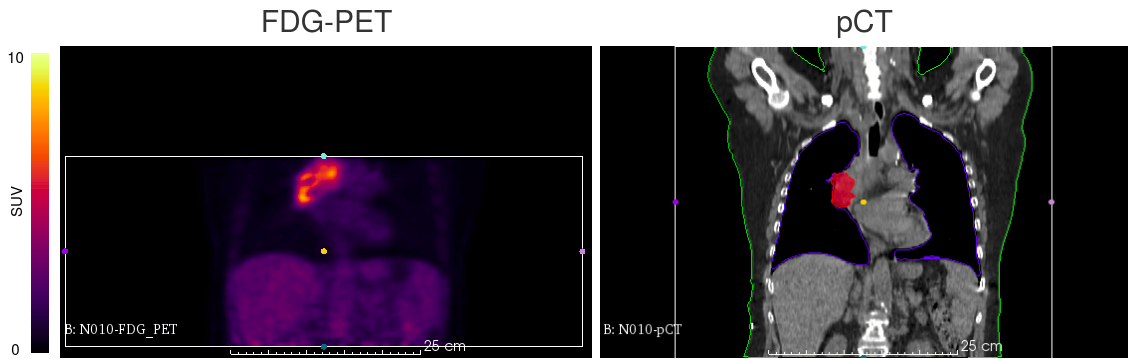
\includegraphics[width=\linewidth]{figures/Data/original/N010-FDG_PET_pCT.png}
    \caption{Single coronal (\textit{x}-\textit{z} plane) slice of FDG-PET and pCT images. White bounding boxes show their respective FOVs. Radiotherapy structure annotations were provided for pCT of which three are shown here -- the patient's body (green), the lungs (dark blue) and the primary tumor (red). The FDG tracer has high specificity to metabolism, resulting in high contrast near the tumor.}
    \label{fig:original_fdgpet_pct}
\end{figure}

In PET image acquisition, a CT scan is usually acquired in the same session whether or not this scan has a separate role, for example, in treatment planning. First, the CT image shows the underlying anatomy for the PET image to be overlaid on it as a contrast map. Second, the material density information captured in the CT scan is used to apply density correction to the recorded PET intensities. The second set of images in the dataset, therefore, includes for each patient an HX4-PET image as well as its accompanying CT scan, both of which are spatially aligned with each other. This CT was acquired using a low radiation dose and is hereafter referred to as \textit{ldCT}. For each patient, the HX4-PET/ldCT scans were acquired on a different day than their corresponding FDG-PET/pCT scans. Both HX4-PET and ldCT images cover approximately the same FOV of the patient's chest. However, the common FOV covered by the HX4-PET/ldCT couple is more focused on the tumor and is smaller in the axial direction compared to that of the FDG-PET/pCT couple. The HX4-PET images have a resolution of 4$\times$4$\times$4 mm$^3$ and the resolution of ldCT is 1.17$\times$1.17$\times$4 mm$^3$. Figure \ref{fig:original_hx4pet_ldct} shows a visualization of sample HX4-PET and ldCT images.

\begin{figure}[h!]
    \centering
    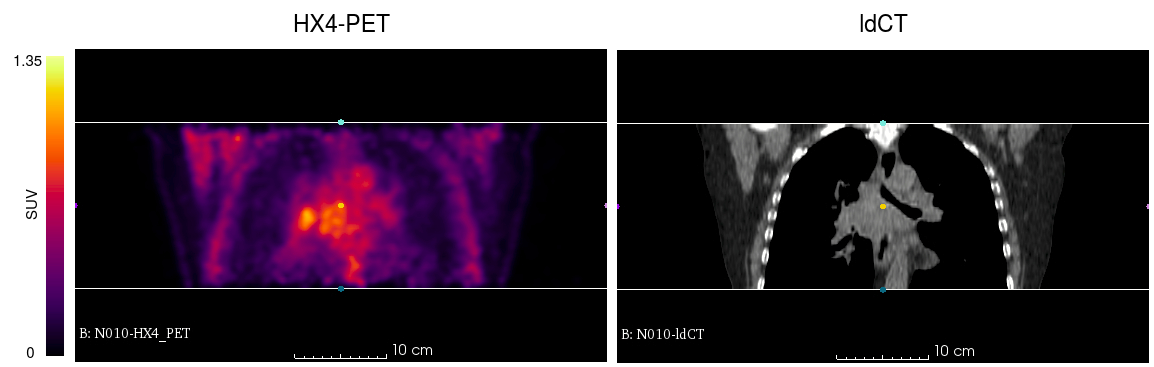
\includegraphics[width=\linewidth]{figures/Data/original/N010-HX4_PET_ldCT.png}
    \caption{Single coronal slice of HX4-PET and ldCT images. Both had similar FOVs. No annotations were provided for the ldCT.}
    \label{fig:original_hx4pet_ldct}
\end{figure}

Voxel intensity values of both pCT and ldCT images are expressed in Hounsfield Units (HU), which relate to the radiodensity of materials. In FDG-PET, the units represent levels of radioactivity emitted from the FDG tracer in different parts of the body as measured by the scanner and are represented in terms of Becquerel per milliliter (Bq/mL, abbreviated as BQML). In HX4-PET, however, intensities are expressed in a different unit called \textit{counts} (abbreviated as CNTS). This unit of PET representation is specific to the manufacturer and the model of the PET/CT scanner (Philips Gemini TF64) that was used for HX4-PET acquisition. Before utilizing the FDG-PET and HX4-PET images for any purpose, their intensities must be converted to a standard and clinically relevant intensity representation -- the Standardized Uptake Value (SUV). SUV calculation is discussed in further detail in \ref{data_proc_phase_1}.


% -----------------------------
\subsection{Image Registration}
Note that the two PET/CT scan pairs -- FDG-PET/pCT and HX4-PET/ldCT -- were acquired on different days for each patient, and because of the differences in patient positioning, they do not spatially align with each other. Having a version of HX4-PET that is aligned with FDG-PET/pCT is essential to serve as the ground truth image for evaluating the GANs as well as for paired training of Pix2Pix. Even et al. \cite{even2017predicting} describe a registration procedure for achieving this alignment. They use a two-step approach where the ldCT is first subjected to rigid alignment followed by non-rigid elastic registration over the pCT. The resulting transformation parameters are then applied to the HX4-PET image.

In addition to the originally acquired scans, the dataset also already includes the registered HX4-PET and ldCT images, and therefore this registration step wasn't needed to be performed. These images are supplied in the \textit{.mhd/.raw} format. The intensity values of the registered HX4-PET are expressed in SUVs, supposedly calculated before the registration process. 

To distinguish the registered HX4-PET from its unregistered counterpart, the two are denoted as \textit{HX4-PET-reg} and \textit{HX4-PET-unreg}, respectively. The term ``HX4-PET" is hereafter used to denote the imaging modality in a general sense and not particularly referring to the registered or unregistered versions of the image. FDG-PET and pCT modalities would be used as inputs to the GAN models and HX4-PET-reg as the ground truth wherever required. Since HX4-PET-reg contains artificial deformations and is likely to contain registration errors as well, the HX4-PET-unreg images instead would be used in the unpaired CycleGAN training. The \textit{unregistered} ldCT, \textit{ldCT-unreg}, would play a crucial role in our modified CycleGAN system, described further in \ref{cyclegan}. However, the \textit{registered} ldCT would not be required anymore beyond this point since its sole purpose was to aid in the registration of HX4-PET, and is thus discarded.


% -------------------------------------
\subsection{Data Preparation Procedure}
\label{Data_Processing}
The dataset needed to be prepared by converting it into a form that could be used for GAN training. The data preparation process can be broken down into two phases, which are elaborated in the following paragraphs. 


\subsubsection{Loading Images and Converting to Appropriate Representation}
The first phase of data preparation involves loading the various images to the computer memory and converting them to a suitable representation. The \textit{PyDicom} library is used for reading the DICOM series along with their metadata, and the \textit{SimpleITK} library for the programmatic representation and manipulation for the loaded images. In certain specialized processing tasks, such as PET SUV calculation and RTstruct conversion, parts of code from this \footnote{HECKTOR 2020 Challenge repository: \url{https://github.com/voreille/hecktor}. It contains utility code created as part of the HECKTOR PET/CT segmentation challenge \cite{andrearczyk2020overview} by its respective authors.} public repository are used to ensure the correctness of the implementation.  

\vspace{4mm}
\noindent
\textit{SUV Calculation:} First, The FDG-PET and HX4-PET-unreg intensity values are converted into the SUV scale. When the intensity units are expressed as BQML, as with all FDG-PET images here, the patient's body weight as well as imaging parameters including the decay time and the total administered dose of the radiotracer are required to calculate the SUV. Equation \ref{BQML_to_SUV} shows the conversion formula. 
\begin{equation}
    SUV = \frac{BQML * 1000 * Weight}{Dose * 2^{-t/\tau}} 
    \label{BQML_to_SUV}
\end{equation}
where $\frac{1}{2^{-t/\tau}}$ is the decay correction factor at time of acquisition \textit{t}, given the half-life $\tau$ of the radiotracer. The values for the patient's weight, administered dose and decay parameters are stored in the DICOM image series as metadata. 

HX4-PET-unreg images, however, are represented in terms of the non-standard CNTS units here, for reasons discussed earlier in \ref{Original_Scans}. CNTS-to-SUV conversion is performed using the formula implemented here \footnote{Implementation of CNTS-to-SUV conversion from the HECKTOR source code: \url{https://bit.ly/3wbtGgW}}.

\vspace{4mm}
\noindent
\textit{Conversion of RTstruct Contours to Binary Masks:} RTstruct is the format defined in the DICOM standard for storing radiotherapy-related annotations (known as ``radiotherapy structure sets") as a set of contour points. The RTstruct file is stored separately from the scans. Since the pCT is used for annotating these contours during radiotherapy treatment planning, the physical coordinate system of the pCT scan is the reference frame for the contour points. Of all the different objects annotated in the pCT scan, we select only the contours for the primary tumor and the patient's body, and convert them to binary masks. Each of these resulting masks has the same 3D size and resolution as the pCT image. The tumor mask would be needed during the clinical evaluation of the hypoxia maps predicted by the models, whereas the body mask would be required during model training to mask away and remove out-of-body objects that are visible in the scans, for instance, the scanner table. The algorithm used for RTstruct-to-binary-mask conversion can be found here \footnote{Implementation of RTstruct-to-binary mask conversion from the HECKTOR source code: \url{https://bit.ly/2RnNI9t}}.

\begin{figure}[h!]
    \centering
    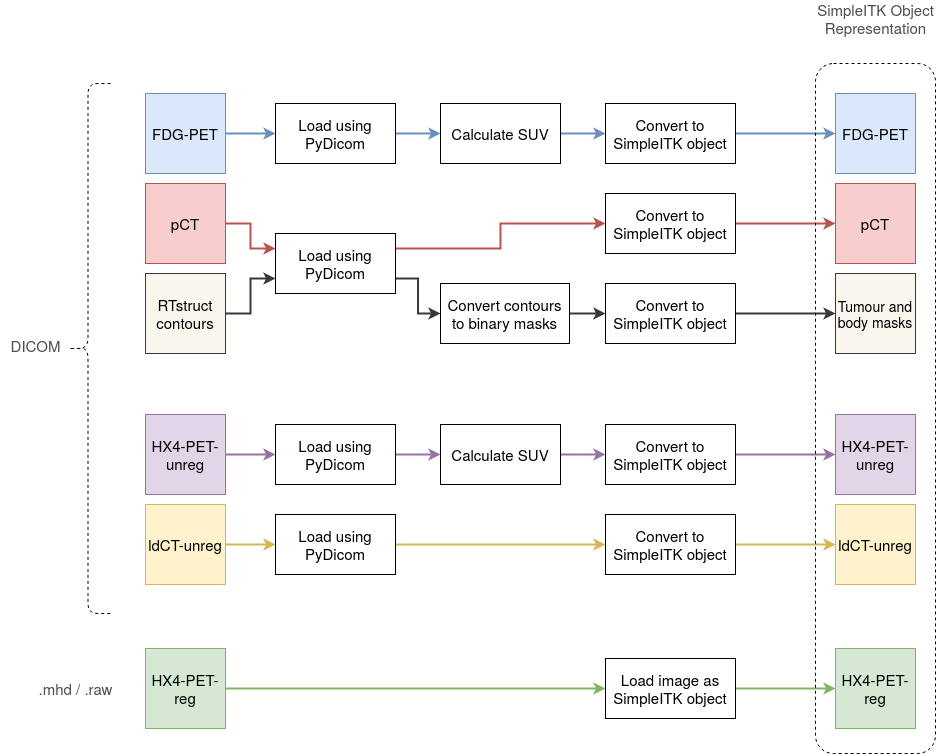
\includegraphics[width=0.9\linewidth]{figures/Data/data_processing_overview-step_1.png}
    \caption{Overview of the first phase of data processing. Images are loaded from storage and converted into a suitable representation for further processing.}
    \label{fig:data_proc_overview_1}
\end{figure}

Following this, the FDG-PET, HX4-PET-unreg, pCT and the tumor and body masks are converted to SimpleITK objects in Python. The ldCT-unreg is also loaded using PyDicom and converted to this representation. HX4-PET-reg, stored in \textit{.mhd/.raw} format containing pre-computed SUV values, is directly loaded into a SimpleITK object. Figure \ref{fig:data_proc_overview_1} shows a visual overview of these steps.


\subsubsection{Cropping and Resampling}
\begin{figure}[h!]
    \centering
    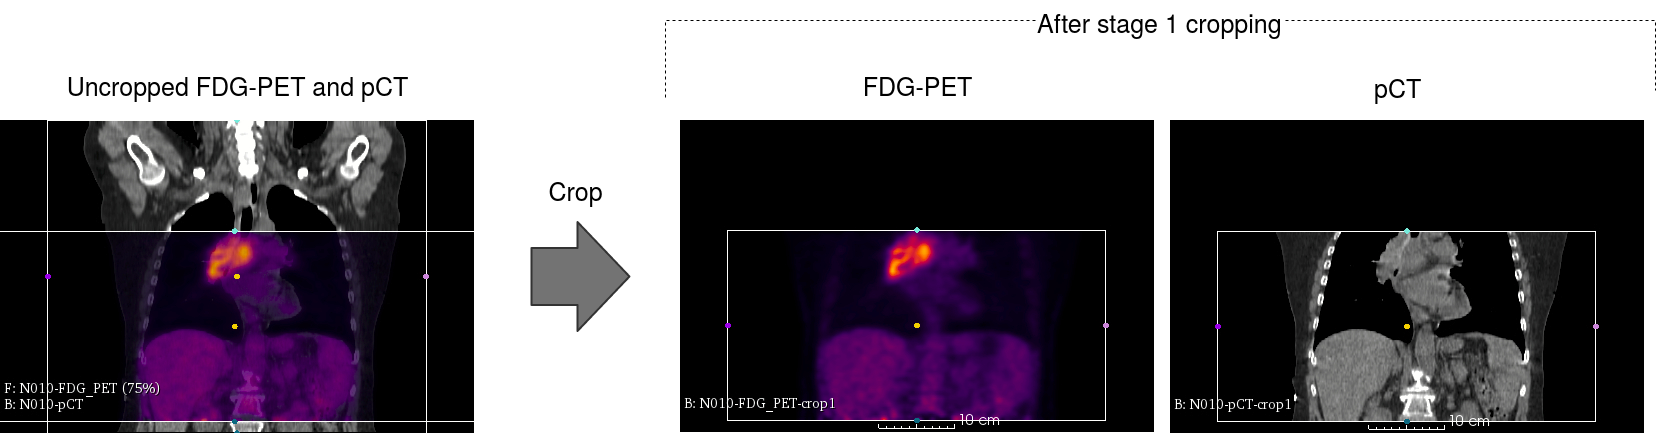
\includegraphics[width=\linewidth]{figures/Data/fdgpet_pct_crop1/N010-FDG_PET_pCT-uncropped_crop1.png}
    \caption{Stage 1 cropping of FDG-PET, pCT and the tumor and body masks (not shown here) to a common FOV. Uncropped FDG-PET and pCT are overlaid to show the overlap of their FOVs.}
    \label{fig:fdg_pet_pct_crop1}
\end{figure}

\begin{figure}[h!]
    \centering
    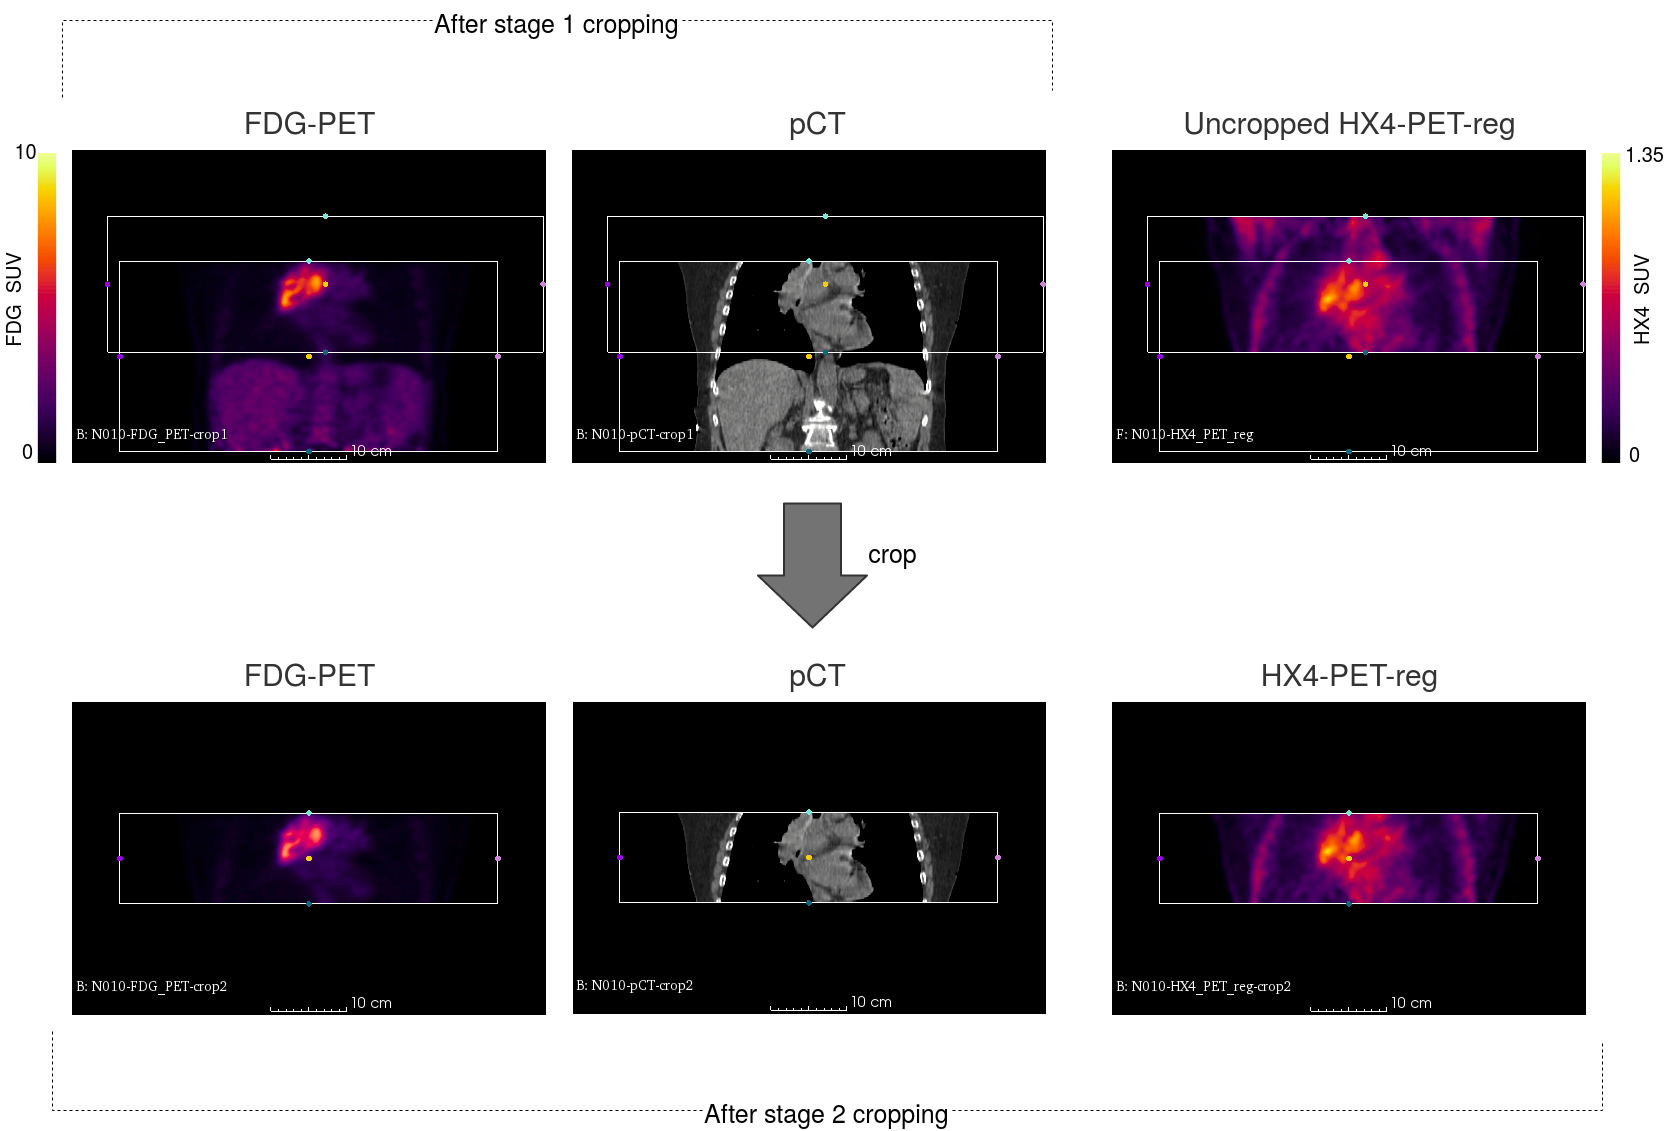
\includegraphics[width=\linewidth]{figures/Data/fdgpet_pct_hx4petreg_crop2/N010-fdgpet_pct_hx4petreg-uncropped_crop2.png}
    \caption{Stage 2 cropping of the input images (FDG-PET and pCT), the masks (tumor and body, not shown here) and the ground truth (HX4-PET-reg) to a common FOV. All FOVs are displayed to show their overlap.}
    \label{fig:fdgpet_pct_hx4petreg_crop2}
\end{figure}

The second phase of data processing involves cropping and resampling the loaded images. A standard resampling resolution of 1$\times$1$\times$3 mm$^3$ is used. Cropping is performed in a progressive manner as described in the following steps: 

\begin{enumerate}
    \item \textit{Cropping and resampling FDG-PET, pCT and masks:} As shown earlier in \ref{Original_Scans}, the FOVs of FDG-PET and pCT are different. Both images must be cropped such that each of them would contain the same FOV of the patient. This is accomplished by determining the 3D volumetric intersection of their FOVs and then cropping the images to this 3D bounding box. Resampling is performed immediately following this. The tumor and body masks share the same FOV with pCT, and are, therefore, cropped in the same way as pCT. This step corresponds to the \textit{Stage 1} cropping of FDG-PET, pCT and the masks. Figure \ref{fig:fdg_pet_pct_crop1} illustrates this step.

    \item \textit{Cropping and resampling HX4-PET-unreg and ldCT-unreg:} The same process of cropping to common FOV followed by resampling is performed on HX4-PET-unreg and ldCT-unreg images. This corresponds to the \textit{Stage 1} cropping of HX4-PET-unreg and ldCT-unreg.

    \item \textit{Resampling HX4-PET-reg:} The HX4-PET-reg image is then only resampled to the standard resolution.

    \item \textit{Cropping the input images, the masks and the ground truth image to common FOV:} Furthermore, the two input images (FDG-PET and pCT), the two masks, and the ground truth image (HX4-PET-reg) are cropped to the common FOV shared across them. The is required because although HX4-PET-reg is spatially aligned with the input images and shares the same physical reference frame with them (due to registration), its FOV is different. This step corresponds to the \textit{Stage 2} cropping, and is visualized in Figure \ref{fig:fdgpet_pct_hx4petreg_crop2}.
\end{enumerate}

\begin{figure}[h!]
    \centering
    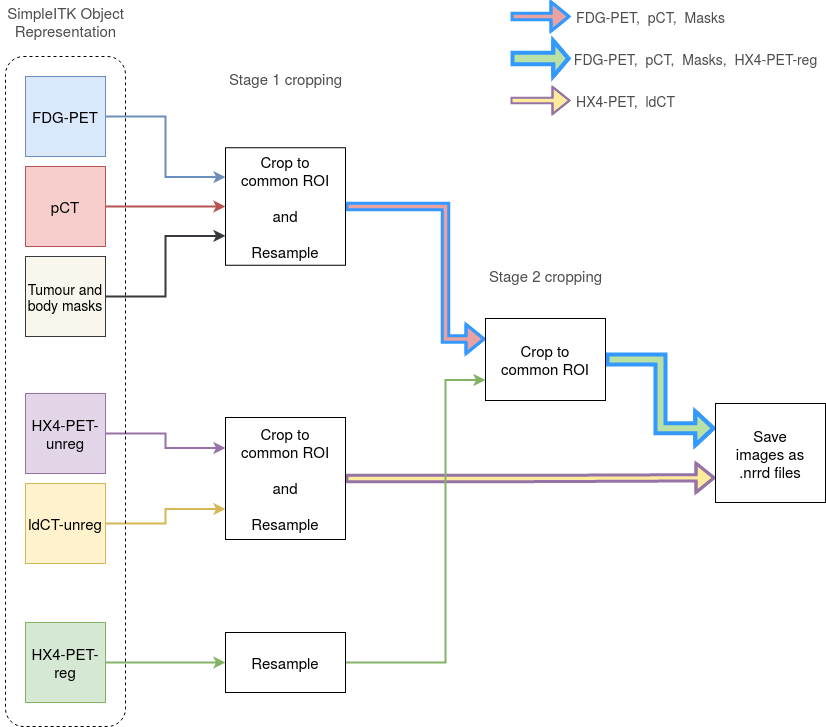
\includegraphics[width=0.8\linewidth]{figures/Data/data_processing_overview-step_2.png}
    \caption{Overview of the second phase of data processing.}
    \label{fig:data_proc_overview_2}
\end{figure}

Finally, all the processed images are saved as \textit{.nrrd} files. The NRRD format allows the storage of N-dimensional raster images along with their spatial information, including voxel spacing (resolution) and physical coordinates of the origin, in a single file. Figure \ref{fig:data_proc_overview_2} shows an overview of the second phase of data processing discussed thus far. The dataset is then split into a training set and a validation set. The training set is comprised of data from the \textit{PET-Boost} clinical trial (15 patients), and the validation set consists of data from the \textit{Nitroglycerin} trial (19 patients). 



%%%%%%%%%%%%%%%%%%%%%%%%%%%%%%%%%%%%%%%%%%%%%%%%%%%%%%%%%%%%%%%%%%%%%%%%%%%%%%%%%%%%%%%%%%%%%%%%%%%%%%%%%%%%%%%%%%%%%%%%%%%%%%%%%%%%%%%%%%%%%%%
\section{GAN Systems}
\label{GAN_Systems}
This section describes the image translation GAN systems used in our study. Unless explicitly mentioned otherwise, domain \textit{A} is used throughout this section to denote the domain of valid multimodal FDG-PET/pCT images, and \textit{B} to denote the domain of HX4-PET images. Synthetic HX4-PET is referred to as \textit{HX4-PET-syn}.


% ------------------
\subsection{Pix2Pix}
\label{pix2pix}
The Pix2Pix framework provides a straightforward image translation method, provided that the domain \textit{A} and domain \textit{B} images in the training dataset are paired, i.e. they are spatially aligned and have pixel-wise correspondence. Given a task of translating a domain \textit{A} image to its equivalent domain \textit{B} image, it is first assumed that an \textit{A}$\rightarrow$\textit{B} mapping exists. The generator models this relationship between the domains, and the discriminator models the conditional probability that an image belongs to domain \textit{B}, given its domain \textit{A} counterpart. During training, the conditional discriminator evaluates the generated domain \textit{B} images, and its adversarial feedback is used to improve the generator's performance. Additionally, Pix2Pix includes an element-wise loss to directly enforce similarity between the synthetic and the ground truth domain \textit{B} images. For a generator $G$ and a discriminator $D$, Equations \ref{eq:pix2pix_loss_components} show the components of each of their loss functions. 

\begin{equation}
    \begin{aligned}
    L(G) &= L_{adv}(G) + \lambda_{elem} L_{elem}(G) \\
    L(D) &= L_{adv}(D)
    \end{aligned}
    \label{eq:pix2pix_loss_components}
\end{equation}
The generator loss has two terms -- an adversarial loss $L_{adv}(G)$ and an element-wise loss $L_{elem}(G)$. The discriminator loss is a single adversarial loss $L_{adv}(D)$ which is the adversarial counterpart of $L_{adv}(G)$. For the generator, $L_{adv}(G)$ can be viewed as a ``structured" loss that is learned from the data itself as a result of the adversarial setting and can produce images with sharp and fine structures, whereas $L_{elem}(G)$ emphasizes on the fidelity of larger and lower-frequency components of the images. The hyperparameter $\lambda_{elem}$ can be used to adjust the balance of importance between the two terms depending on the specific application.

We use the least-squares version of the adversarial loss, instead of the original cross-entropy loss, as it is known to improve training stability \cite{mao2017least}. Similar to the original Pix2Pix framework \cite{isola2017image}, we implement $L_{elem}(G)$ using voxel-wise L1 loss. Equations \ref{eq:pix2pix_loss_expansion} show the expansion of each of these loss terms.

\begin{equation}
    \begin{aligned}
    L_{adv}(G) &= E_{x \sim p_{data}(x)} [(1 - D(x, G(x)))^2]  \\
    L_{adv}(D) &= E_{x \sim p_{data}(x)} [D(x, G(x))^2] + E_{x,y \sim p_{data}(x,y)} [(1 - D(x,y))^2] \\
    L_{elem}(G) &= E_{x,y \sim p_{data}(x,y)} [|| y - G(x) ||_1]  \\
    \end{aligned}
    \label{eq:pix2pix_loss_expansion}
\end{equation}

where $x$ and $y$ are random variables representing paired samples from domain \textit{A} and \textit{B}, respectively. During training, $G$ and $D$ are updated in an alternating fashion. For a given $D$, $G$ learns to synthesize images that $D$ would wrongly classify as real data samples, with value 1 (optimizing for $L_{adv}(G)$), while simultaneously aiming for voxel-wise fidelity of its output with the ground truth (optimizing for $L_{elem}(G)$). Whereas, for a given $G$, $D$ learns to correctly classify the synthetic samples as 0 and the real samples as 1 (thereby optimizing for $L_{adv}(D)$).

\begin{figure}[h!]
    \centering
    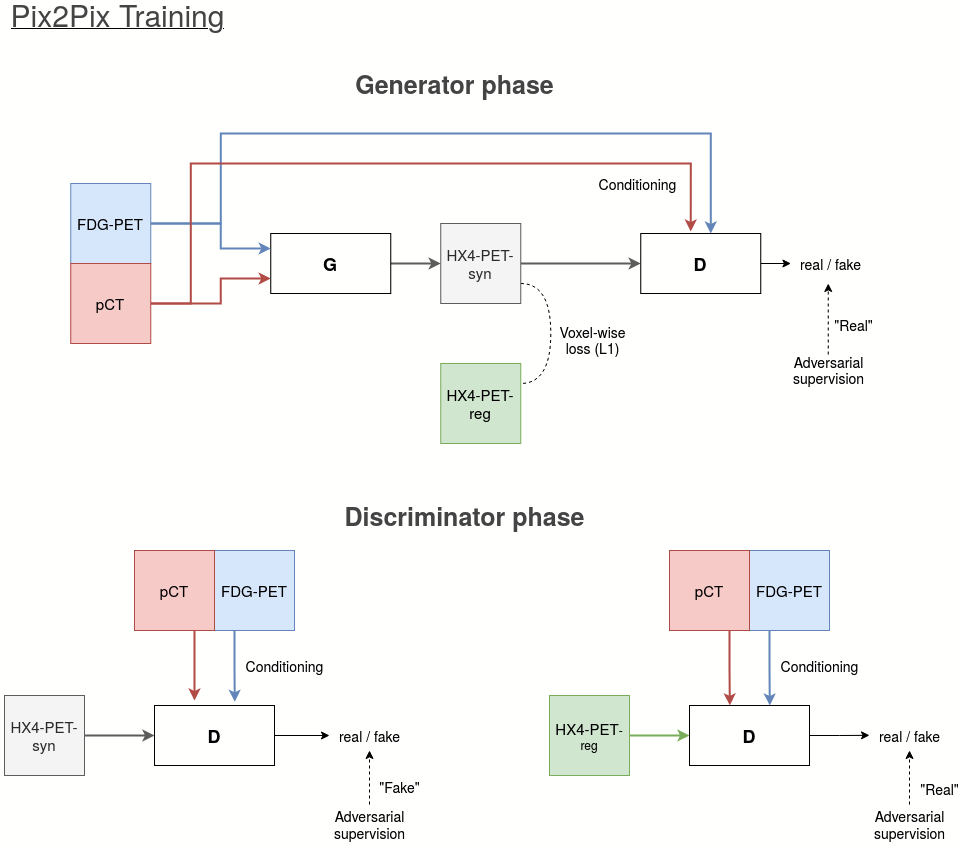
\includegraphics[width=0.9\linewidth]{figures/GANs/Pix2Pix.png}
    \caption{Pix2Pix training phases. \textit{G} and \textit{D} are updated in an alternating manner. In practice, FDG-PET and pCT images are stacked channel-wise and given as input to \textit{G}. And the discriminator conditioning is implemented by stacking channel-wise the HX4-PET-reg or HX4-PET-syn with FDG-PET and pCT.}
    \label{fig:pix2pix}
\end{figure}{}

We apply Pix2Pix to our translation problem in a 3D manner on the volumetric medical images. Given the FDG-PET and pCT images as input and the corresponding HX4-PET-reg images as the target, the model is trained to generate HX4-PET-syn images representative of the target domain. Figure \ref{fig:pix2pix} shows a schematic of the generator and discriminator training phases.


% -------------------
\subsection{CycleGAN}
\label{cyclegan}

CycleGAN addresses unpaired image translation problems where \textit{A}-\textit{B} image pairs are not provided in the training set. It is first assumed that there exists some relationship between domain \textit{A} and domain \textit{B} and that this relationship is bijective in nature. In other words, for an \textit{A}$\rightarrow$\textit{B} transformation, an inverse \textit{B}$\rightarrow$\textit{A} transformation exists. CycleGAN aims at modeling these two mappings simultaneously by incorporating cycle-consistency with the principal idea being that translating an image to another domain and then back to its original domain should yield the same image.  The GAN system consists of two generators -- $G_{AB}$ and $G_{BA}$ -- that implement the \textit{A}$\rightarrow$\textit{B} and \textit{B}$\rightarrow$\textit{A} mappings, respectively. Two discriminators $D_B$ and $D_A$ are adversarially coupled with the respective two generators. Note that, unlike Pix2Pix, discriminators in CycleGAN are not conditioned on input images as this is not possible with unpaired training data. Equations \ref{eq:cyclegan_naive_loss_components} show the generator and discriminator loss terms.

\begin{equation}
    \begin{aligned}
    L(G_{AB}, G_{BA}) &= L_{adv}(G_{AB}) + L_{adv}(G_{BA}) + \lambda_{cyc} L_{cyc}(G_{AB}, G_{BA}) \\[1mm]
    L(D_B, D_A) &= L_{adv}(D_B) + L_{adv}(D_A)
    \end{aligned}
    \label{eq:cyclegan_naive_loss_components}
\end{equation}
The adversarial loss term $L_{adv}(G_{AB})$ of $G_{AB}$ is coupled with $L_{adv}(D_B)$ of $D_B$ and encourages $G_{AB}$ to produce images resembling domain \textit{B} samples. Similarly, $L_{adv}(G_{BA})$ and $L_{adv}(D_A)$ are counterparts of each other and drive $G_{BA}$ to produce images indistinguishable from domain \textit{A}. It would be possible for a generator to satisfy its adversarial constraints by translating its input image from its source domain to just \textit{any} image that would seem like a sample from its target domain, whether or not the translated image preserves the contents of the input image. The cycle-consistency term $L_{cyc}(G_{AB}, G_{BA})$, therefore, acts as an indirect content-preservation criterion that constrains $G_{AB}$ and $G_{BA}$ to preserve the high-level structure across translation, thereby complementing the adversarial losses. The hyperparameter $\lambda_{cyc}$ is used to adjust the relative importance given to cycle-consistency loss. 

Let $x \sim p_{data}(x)$ represent the random variable associated with domain \textit{A} following a distribution $p_{data}(x)$, and $y \sim p_{data}(y)$ be the random variable associated with the domain \textit{B} distribution. Equations \ref{eq:cyclegan_naive_loss_expansion} show each of the loss terms in expanded form.
\begin{equation}
    \begin{aligned}
    L_{adv}(G_{AB}) &= E_{x \sim p_{data}(x)} [(1 - D_B(G_{AB}(x)))^2]  \\[1mm]
    L_{adv}(D_B) &= E_{x \sim p_{data}(x)} [D_B(G_{AB}(x))^2] + E_{y \sim p_{data}(y)} [(1 - D_B(y))^2] \\[4mm]
    L_{adv}(G_{BA}) &= E_{y \sim p_{data}(y)} [(1 - D_A(G_{BA}(y)))^2]  \\[1mm]
    L_{adv}(D_A) &= E_{y \sim p_{data}(y)} [D_A(G_{BA}(y))^2] + E_{x \sim p_{data}(x)} [(1 - D_A(x))^2] \\[4mm]
    L_{cyc}(G_{AB}, G_{BA}) &= E_{x \sim p_{data}(x)} [|| x - G_{BA}(G_{AB}(x)) ||_1]  \\
                            &+ E_{y \sim p_{data}(y)} [|| y - G_{AB}(G_{BA}(y)) ||_1] 
    \end{aligned}
    \label{eq:cyclegan_naive_loss_expansion}
\end{equation}
Cycle-consistency loss $L_{cyc}(G_{AB}, G_{BA})$ encourages a reconstructed image to be as close as possible to its original image in L1 sense, and is applied to both \textit{A}$\rightarrow$\textit{B}$\rightarrow$\textit{A} and \textit{B}$\rightarrow$\textit{A}$\rightarrow$\textit{B} cycles. Figure \ref{fig:cyclegan_concept} shows a conceptual visualization of CycleGAN training.

\begin{figure}
    \centering
    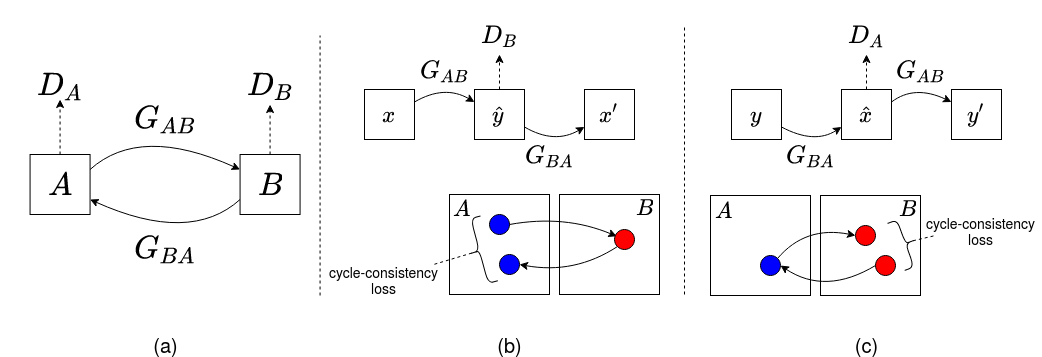
\includegraphics[width=\textwidth]{figures/GANs/cyclegan_concept.png}
    \caption{Simplified representation of CycleGAN training, figure adapted from the original paper \cite{zhu2017unpaired} with notations changed. (a) $G_{AB}$ models \textit{A}$\rightarrow$\textit{B} mapping and $G_{BA}$ its inverse. $D_B$ and $D_A$ are domain \textit{B} and \textit{A} discriminators, respectively. (b) In the \textit{A}$\rightarrow$\textit{B}$\rightarrow$\textit{A} cycle, a domain \textit{A} image $x$ is translated to a representation \textit{$\hat{y} = G_{AB}(x)$} in domain \textit{B}, which is evaluated by $D_B$. It is then used to obtain a reconstruction $x' = G_{BA}(G_{AB}(x))$ of the original image $x$ which is encouraged by the cycle-consistency to be close to $x$. (c) The \textit{B}$\rightarrow$\textit{A}$\rightarrow$\textit{B} cycle.}
    \label{fig:cyclegan_concept}
\end{figure}


\subsubsection{CycleGAN-naive: Default CycleGAN applied to HX4-PET synthesis problem}
We investigate CycleGAN for unpaired translation of FDG-PET/pCT to HX4-PET. The term ``unpaired" can be used at two levels here -- the patient level and the voxel level. At the patient level, our dataset includes all three image modalities for each patient. The training data used for the CycleGAN is patient-level unpaired, meaning the \textit{A}-\textit{B} image correspondence information is not used, and both domain \textit{A} and domain \textit{B} samples are independently shuffled while training. At the voxel level, the registered HX4-PET-reg images are spatially aligned input-target paired data, whereas the unregistered images -- HX4-PET-unreg -- are devoid of any artificial deformations and imperfections that are related to registration. We, therefore, use HX4-PET-unreg images as the set of domain \textit{B} samples which results in our CycleGAN training data being unpaired at the voxel level as well. The default CycleGAN framework naively applied to our use case is henceforth referred to as \textit{CycleGAN-naive}. Figure \ref{fig:cyclegan_naive} shows a schematic of the generator and discriminator training phases of CycleGAN-naive. 

\begin{figure}[h!]
    \centering
    \makebox[\textwidth][c]
    {
        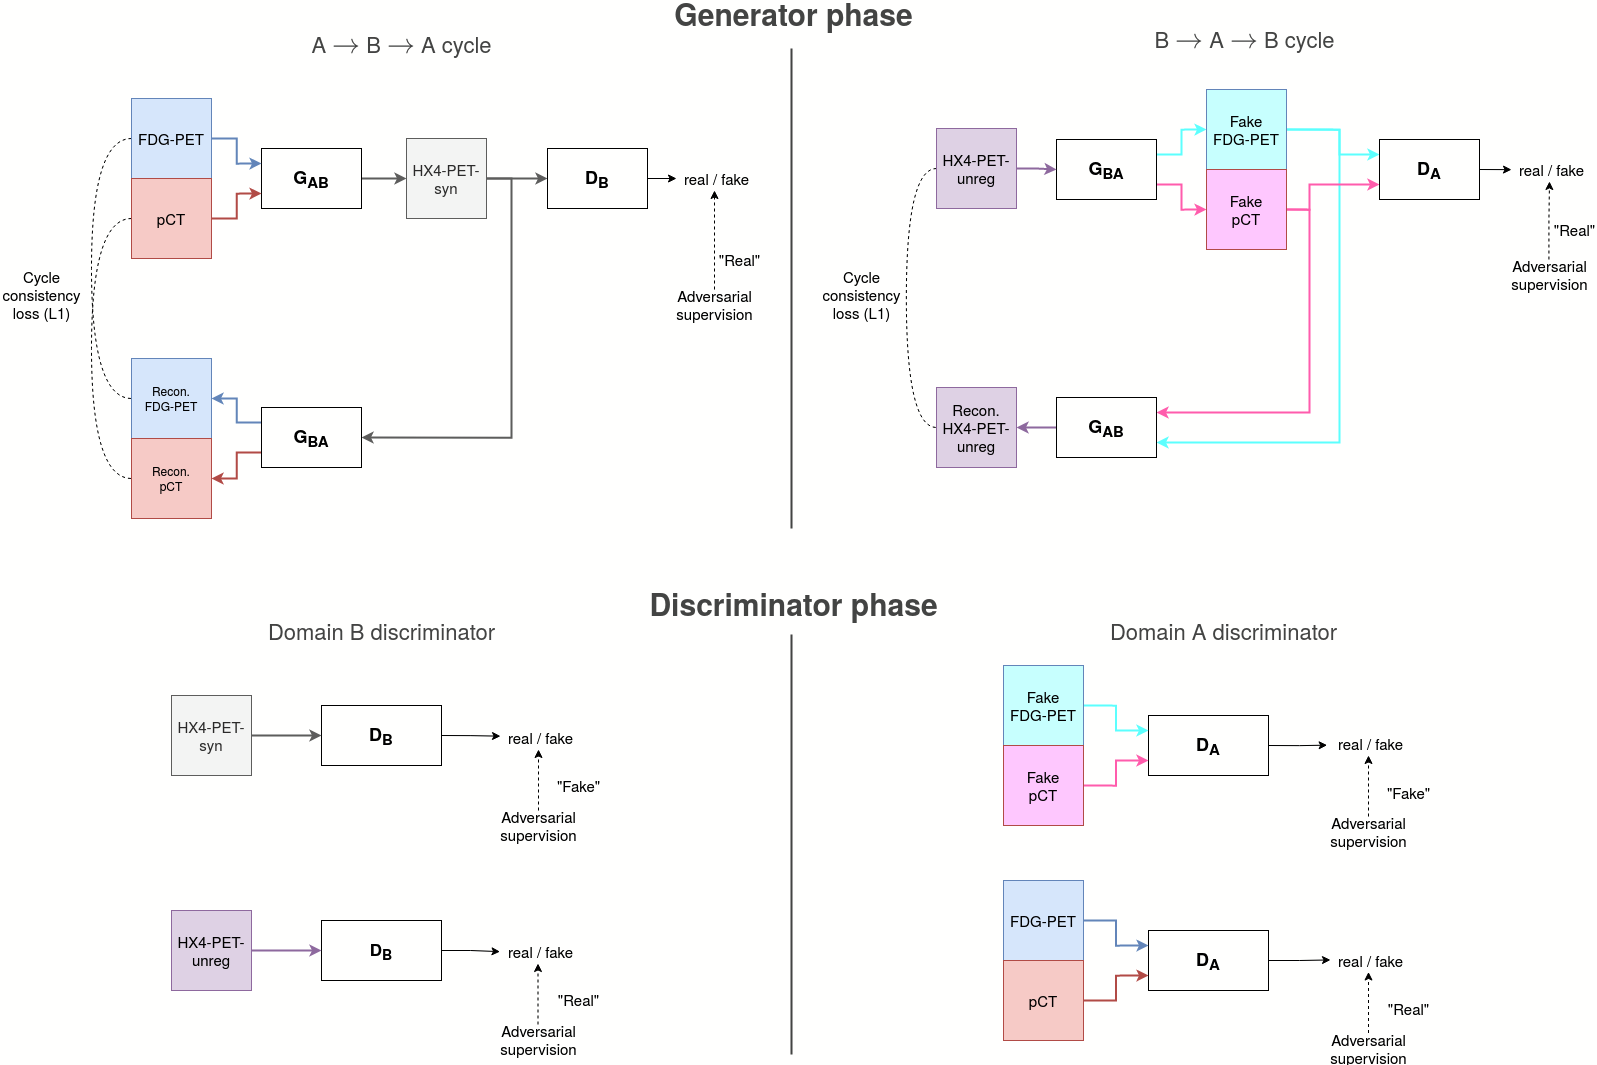
\includegraphics[width=1.5\linewidth]{figures/GANs/CycleGAN-naive.png}
    }
    \caption{CycleGAN-naive training phases. The generators and discriminators are updated in an alternating manner.}
    \label{fig:cyclegan_naive}
\end{figure}{}

We argue that CycleGAN-naive has several drawbacks and therefore, it is not an optimal implementation of CycleGAN for our task. In the \textit{A}$\rightarrow$\textit{B}$\rightarrow$\textit{A} cycle, $G_{AB}$ takes as input FDG-PET and pCT to output HX4-PET-syn, and $G_{BA}$ uses HX4-PET-syn to reconstruct FDG-PET and pCT. The learning task of $G_{AB}$ is realistic since hypoxia patterns can be reliably predicted from the inputs, and therefore, has a physiological basis (see Section \ref{Related_Work-hypoxia_prediction}). However, the learning task of $G_{BA}$ is not reasonable. It is not possible to precisely predict a patient's anatomy (CT) as well as their metabolism levels (FDG-PET) from just the hypoxia information, and the CT modality is of more concern to our discussion. A CT image contains highly detailed structural information with sharp and fine features, whereas PET images are functional heatmaps having blurred and diffused characteristics. $G_{BA}$ cannot accurately rebuild pCT from HX4-PET-syn unless $G_{AB}$ encodes the CT information into the latter in the form of noise. But then, the HX4-PET-syn image would not resemble a clinically acquired HX4-PET scan. Therefore, cycle-consistency constraint conflicts with the domain \textit{B} adversarial criterion instead of complementing it. Now looking at the \textit{B}$\rightarrow$\textit{A}$\rightarrow$\textit{B} cycle, the task of $G_{BA}$ is to compute realistic FDG-PET and pCT when given only the real HX4-PET-unreg image, which it can perform, especially for pCT, by hallucinating the patient's anatomy. However, in that case, $G_{AB}$ would be given this fake information to precisely reconstruct the HX4-PET-unreg. Because the task of $G_{AB}$ is to correctly predict hypoxia based on given CT (and FDG-PET) information, it is unreasonable to provide it with fake anatomical information and expect it to predict hypoxia patterns from it that match the real HX4-PET-unreg. In this cycle as well, contradictions across the learning objectives exist. The fundamental assumption made by CycleGAN regarding the existence of a bijective relationship between domains \textit{A} and \textit{B} does not hold in our data, and the resulting images are likely to be highly inaccurate and not representative of the patient's condition. Based on these reasons, we believe that CycleGAN, in its default form, cannot tackle this translation problem and that a more intelligent strategy is required.


\subsubsection{CycleGAN-balanced: An improved design}
We propose a custom design improvement to CycleGAN training to make the system more optimized for our use case. We utilize the fact that an HX4-PET scan is always acquired together with a CT scan which, in our dataset, is a low-dose CT (ldCT). For this system, the training process is unpaired similar to CycleGAN-naive, and the ldCT-unreg images are included in the training data accompanying their corresponding HX4-PET-unreg images. 

We begin by slightly altering what the domains \textit{A} and \textit{B} denote here -- let \textit{A} be the domain of FDG-PET images and \textit{B} of HX4-PET images. The CT images -- pCT and ldCT -- are then considered to be ``supporting" images that provide \textit{anatomical context} to the generators. Note that pCT has spatial correspondence only with FDG-PET, and ldCT-unreg is aligned only with HX4-PET-unreg. Now, the task of each generator is to take as input a PET image from its source domain and compute its target domain PET image, while being supplied anatomical context using the \textit{available} CT image (i.e the one that is aligned with the source domain PET). To elaborate on this, consider the two cycles separately: 

\begin{itemize}
    \item \textit{A$\rightarrow$B$\rightarrow$A cycle}: Here, pCT is the available CT image which accompanies the FDG-PET. In \textit{A}$\rightarrow$\textit{B} translation, $G_{AB}$ uses the two images and computes HX4-PET-syn. In \textit{B}$\rightarrow$\textit{A} translation, $G_{BA}$ now \textit{reuses} the pCT as a support image along with the HX4-PET-syn (note that the two are aligned) to reconstruct FDG-PET. The pCT provides the same anatomical context for FDG-PET reconstruction as it did for HX4-PET-syn prediction. The cycle-consistency loss is computed between the FDG-PET and its reconstructed version. If the HX4-PET-syn represents a plausible hypoxia prediction, then the FDG-PET can be recovered from it up to a great extent since both have an underlying physiological relationship. Therefore, the adversarial loss would drive $G_{AB}$ to produce realistic HX4-PET-syn image and the cycle-consistency loss would encourage this image to be representative of the patient's physiology. 
    
    \item \textit{B$\rightarrow$A$\rightarrow$B cycle}: In this case, ldCT-unreg is the available CT image that is coupled with the HX4-PET-unreg. In \textit{B}$\rightarrow$\textit{A} translation, $G_{BA}$ uses these two images to compute a synthetic FDG-PET. In \textit{A}$\rightarrow$\textit{B} translation, $G_{AB}$ reuses the ldCT-unreg and together with the synthetic FDG-PET (note that the ldCT-unreg and the synthetic FDG-PET are aligned), it reconstructs HX4-PET-unreg. Cycle-consistency is applied between the original and reconstructed HX4-PET-unreg. The same ldCT-unreg image provides anatomical context for FDG-PET synthesis and for HX4-PET-unreg reconstruction, and if the synthetic FDG-PET represents plausible metabolism patterns, then HX4-PET-unreg can be mostly recovered. In this cycle as well, the adversarial and cycle-consistency objectives would behave in a mutually reinforcing manner.
\end{itemize}

The introduction of CT as an \textit{input} to both the generators creates a balance between the complexities of the \textit{A}$\rightarrow$\textit{B} and \textit{B}$\rightarrow$\textit{A} mappings since none of them involves \textit{predicting} fake CT information, while still using completely unpaired training data. Unlike CycleGAN-naive, the \textit{A}$\rightarrow$\textit{B} and \textit{B}$\rightarrow$\textit{A} relations are not anymore inverses of each other, in the strict sense of the word. We term this modified design \textit{CycleGAN-balanced}. Figure \ref{fig:cyclegan_balanced} shows a schematic of the training phases of its generators and discriminators.

\begin{figure}[h!]
    \centering
    \makebox[\textwidth][c]
    {
        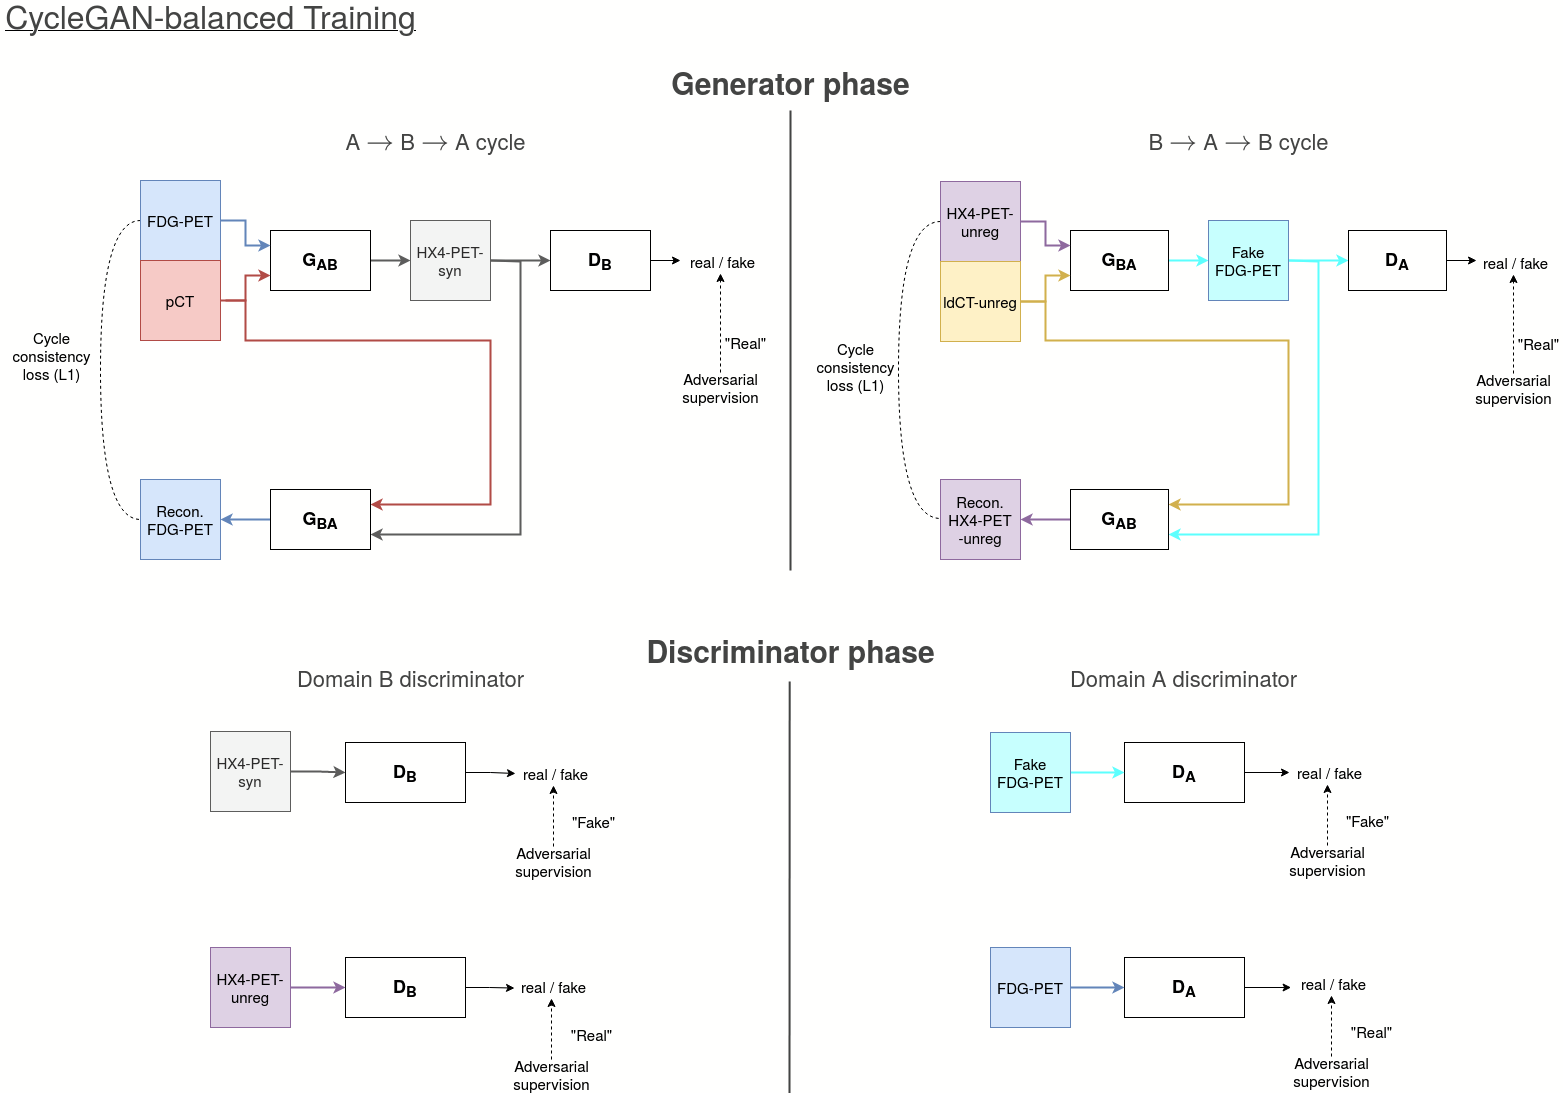
\includegraphics[width=1.5\linewidth]{figures/GANs/CycleGAN-balanced.png}
    }
    \caption{CycleGAN-balanced training phases. \textit{A}$\rightarrow$\textit{B} and \textit{B}$\rightarrow$\textit{A} translation tasks are balanced. The CT images provide anatomical context to the generators. In \textit{A}$\rightarrow$\textit{B}$\rightarrow$\textit{A} cycle, the pCT is used as an input by $G_{AB}$ and then reused by $G_{BA}$. In the \textit{B}$\rightarrow$\textit{A}$\rightarrow$\textit{B} cycle, the ldCT-unreg is the common CT image used by both the generators.}
    \label{fig:cyclegan_balanced}
\end{figure}{}

Low-dose CT scans are characterized by a higher amount of acquisition-related noise compared to routine- or high-dose CT scans (such as planning CT). An additional, possibly desirable, consequence of exposing the two generators to both pCT and ldCT images during training is that the model is likely to learn effectively the relevant anatomical features while disregarding any pCT-specific or ldCT-specific noise signatures. That is, they are likely to generalize over both types of CT images. This is merely a property of CycleGAN-balanced that we make a note of, although we do not investigate this further.


%%%%%%%%%%%%%%%%%%%%%%%%%%%%%%%%%%%%%%%%%%%%%%%%%%%%%%%%%%%%%%%%%%%%%%%%%%%%%%%%%%%%%%%%%%%%%%%%%%%%%%%%%%%%%%%%%%%%%%%%%%%%%%%%%%%%%%%%%%%%%%%
\section{Network Architecture}
\label{network_architectures}
The Pix2Pix, CycleGAN-naive, and CycleGAN-balanced systems share the same generator and discriminator network architectures for the sake of fair comparison. Our design choices of the architectures are based on the specifications of the original Pix2Pix and CycleGAN frameworks \cite{isola2017image, zhu2017unpaired} and involve the 3D equivalent of the 2D spatial operations.

% --------------------
\subsection{Generator}
Each generator network is based on the 3D U-Net architecture \cite{cciccek20163d}. 3D U-Net is a fully convolutional network that takes as input a 3D volumetric image of arbitrary size and can produce an output image of the same size as the input. It consists of an \textit{analysis} path (or encoder) where hierarchical features are progressively extracted from the input image and a \textit{synthesis} path (or decoder) that progressively constructs the output image from the features. A desirable property of the U-Net is its skip connections that transport features of multiple abstraction levels directly into the synthesis path, enabling it to utilize both high- and low-level features in synthesizing the output. In contrast to a U-Net, a traditional encoder-decoder network without any skip-connections must depend on its highest-level features (i.e. features from its ``bottleneck" ). In many image translation problems, the input and target domain images could share a large amount of low-level information. The U-Net is known to produce better quality images in such cases compared to the encoder-decoder architecture \cite{isola2017image}.

Loosely based on the notation used in \cite{isola2017image}, we use \textit{Enc-Ck} to represent an encoder block composed of Convolution-InstanceNorm-LeakyReLU layers where the convolution operation uses \textit{k} 3D kernels of size 4$\times$4$\times$4 voxels, applied with a stride 2$\times$2$\times$2 and zero padding of 1 at each side of the input along each axis. The Leaky ReLU has a negative side slope of 0.2. For the decoder, let \textit{Dec-Tk} represent a block comprising of TransposedConvolution-InstanceNorm-ReLU layers where the 3D upsampling transposed convolution uses \textit{k} kernels of size 4$\times$4$\times$4, stride 2$\times$2$\times$2, and input padding of 1 at each side along each axis. With the given configuration, the encoder downscales the image representation by a factor of 2 at every stage, and the decoder upscales it by the same factor. Our U-Net architecture is then specified in Table \ref{tab:generator_architecture}.

\begin{table}[h!]
    \centering
    \begin{tabular}{|c|c|c|}
        \hline
        \textbf{Encoding Level} & \textbf{Encoder block} & \textbf{Decoder block} \\
        \hline
        1     & Enc-C64          & Dec-T1           \\
        \hline
        2     & Enc-C128         & Dec-T64          \\
        \hline
        3     & Enc-C256         & Dec-T128         \\
        \hline
        4     & Enc-C512         & Dec-T256         \\
        \hline
        5     & Enc-C512         & Dec-T512         \\
        \hline
    \end{tabular}
    \caption{The first encoder block Enc-C64 accepts a two-channel input image and the encoder path processes the image from encoding level 1 to 5. The first decoder block Dec-T512 is in correspondence with the last encoder block Enc-C512, and the decoder path performs computation starting from encoding level 5 to 1, ultimately producing a single channel output image from Dec-T1. An exception to the U-Net's input and output channels appears in CycleGAN-naive, where the generator $G_{BA}$ requires a single channel input and produces a two-channel output.}
    \label{tab:generator_architecture}
\end{table}

There are two exceptions to the aforementioned block notations. The first encoder block (Enc-C64) and the last decoder block (Dec-T1) do not use instance normalization. And, the latter uses the \textit{tanh} activation function to output an image with intensity values bounded within the range (-1, 1). 


% ------------------------
\subsection{Discriminator}
We use the 3D PatchGAN architecture for our discriminators. The network is essentially a convolutional classifier that, instead of computing a single validity score for an image (0 if fake, 1 if real), evaluates independent scores for fixed-size local regions (or patches) of the image. It, therefore, encourages the synthetic images to not only resemble the target domain at the global level but also for its local high-frequency structures to reflect the characteristics of the domain. PatchGAN discriminator of a fixed architecture can take an input image of arbitrary size and produces an output map whose size depends on the input image size, while each output unit's \textit{receptive field} size is constant with respect to the input image. The receptive field size can be increased by increasing the depth of the network.

Let \textit{Ck} denote a block composed on Convolution-InstanceNorm-LeakyReLU where the 3D convolution layer uses \textit{k} kernels of size 4$\times$4$\times$4 and input padding of 1 at each side along each axis, and the Leaky ReLU has a negative side slope of 0.2. The exact discriminator architecture is then shown in Table \ref{tab:discriminator_architecture}. Under this configuration, the receptive field of each output unit is 70$\times$70$\times$70 voxels on the input image.

\begin{table}[h!]
    \centering
    \begin{tabular}{|c|c|}
        \hline
        \textbf{Block number} & \textbf{Discriminator block}\\
        \hline
        1     & C64       \\
        \hline
        2     & C128      \\
        \hline
        3     & C256      \\
        \hline 
        4     & C512      \\
        \hline
        5     & C1        \\
        \hline
    \end{tabular}
    \caption{The first discriminator block C64 takes as input a single channel image (except of $D_A$ of CycleGAN-naive which requires two-channel input). The last block C1 always outputs a single-channel validity score map. Blocks 1, 2 and 3 use a stride of 2$\times$2$\times$2 resulting in a downscaling of the image representation by a factor of 2, whereas blocks 4 and 5 uses a stride of 1$\times$1$\times$1.}
    \label{tab:discriminator_architecture}
\end{table}
As exceptions to the notation, instance normalization is not used in the first and the last blocks. Also, because we use the least-squares adversarial loss, the last block does not include an activation function. The final convolution layer's output map is considered the discriminator's final output.



%%%%%%%%%%%%%%%%%%%%%%%%%%%%%%%%%%%%%%%%%%%%%%%%%%%%%%%%%%%%%%%%%%%%%%%%%%%%%%%%%%%%%%%%%%%%%%%%%%%%%%%%%%%%%%%%%%%%%%%%%%%%%%%%%%%%%%%%%%%%%%%
\section{Model Training}


% --------------------------------------------
\subsection{Overview of the Data Requirements}
\label{data_requirements}
Figure \ref{fig:which_images_where} provides a visual overview of the data requirements of each GAN system to clarify which image type is used where, much of which is covered in detail earlier in Section \ref{GAN_Systems} for each individual GAN. The FDG-PET and pCT images comprise the model input. HX4-PET-reg is the ground truth hypoxia map, and images from the validation set are used to evaluate and track model generalizability during the training process. HX4-PET-reg images from the training set are used to train the paired Pix2Pix model. The unregistered image couples HX4-PET-unreg and ldCT-unreg are required only in the training set, of which only the HX4-PET-unreg is involved in CycleGAN-naive training, whereas both are used in CycleGAN-balanced training.

\begin{figure}[h!]
    \centering
    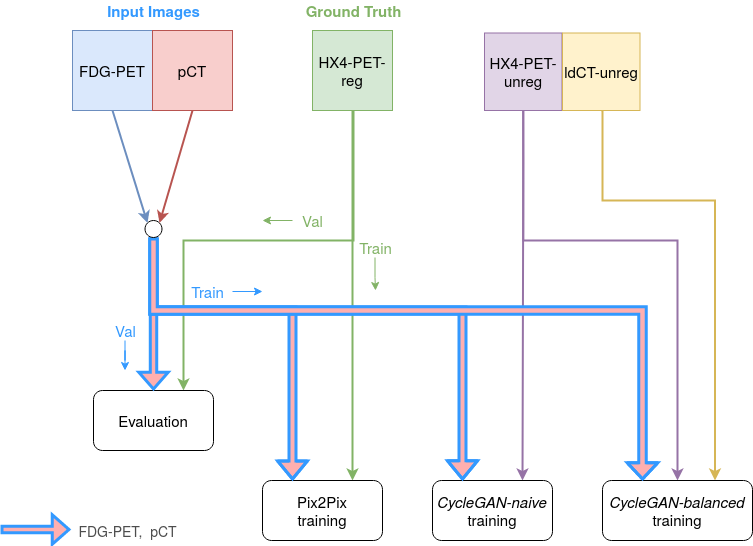
\includegraphics[width=0.8\linewidth]{figures/Data/which_images_where.png}
    \caption{Overview of data requirements of the GAN systems.}
    \label{fig:which_images_where}
\end{figure}


% ----------------------------
\subsection{Training Pipeline}
\label{training_pipeline}

\subsubsection{Data pre-processing and normalization}
Depending on the GAN, the required training images and the body mask are first fetched from their \textit{.nrrd} form into the computer memory. The body mask is applied to pCT, FDG-PET, and HX4-PET-reg (if using), and the out-of-the-body region intensities are set to zero signal value -- i.e. 0 SUV (zero activity) in the PET images and -1024 HU (value for air) in pCT. This body mask was obtained from the pCT (see \ref{Data_Processing}), and therefore, cannot be applied to the unregistered images. When performing unpaired training with HX4-PET-unreg and ldCT-unreg, the latter is used to automatically generate their own body mask via HU thresholding and morphological operations. This new body mask is then applied to HX4-PET-unreg (and ldCT-unreg, if using). Body masking is then followed by normalization. CT intensities are clipped and limited to the HU range [-1000, 2000] and then linearly rescaled to range [-1, 1]. FDG-PET is clipped into the SUV range [0, 15] followed by rescaling to [-1, 1]. In the case of HX4-PET images, following previous related work \cite{even2017predicting}, the SUV values are first divided by the mean SUV of the patient's aorta region. The resulting intensity representation ($\frac{SUV}{SUV_{aorta-mean}}$ ratio) has a special meaning when used in the context of the tumor, wherein it is referred to as the tumor-to-background ratio (TBR). Here, the aorta is considered the ``background" with respect to the tumor. This is a clinically useful intensity representation that has pre-defined standard thresholds \cite{zegers2013hypoxia} and can, hence, be used for hypoxia quantification during image evaluation (described further in Section \ref{Evaluation_Methods}). We perform this conversion step at the beginning of the training pipeline, instead of during the evaluation stage, because the aorta annotation was not provided in the dataset which makes it impossible to compute the $SUV_{aorta-mean}$ value directly from the HX4-PET images. These values were instead provided for each patient directly in a separate file, and we had to depend on them for SUV $\leftrightarrow$ TBR conversion throughout the training and evaluation stages. Following the conversion of the body masked HX4-PET images into this intensity unit, the intensities are clipped to the range [0, 3] and then rescaled to [-1, 1]. The aforementioned clipping ranges for FDG-PET SUV and HX4-PET $\frac{SUV}{SUV_{aorta-mean}}$ are used because they covered most of the intensity variation in their respective images, especially in the tumor area.

\subsubsection{Patch-based training}
We use a patch-based training approach to cope with the high memory requirements of the 3D GANs and with the small size of the training set. For each pre-processed image, a single 3D patch is extracted from the image and is used to feed the model. The body mask is used to limit patch sampling to the body region to avoid extracting patches from the background. Patches from the input images (FDG-PET and pCT) are sampled randomly with a uniform random distribution over the body region. Then, depending on whether the training is paired or unpaired, a suitable \textit{patch propagation} strategy is used to obtain a corresponding patch from the given HX4-PET image.

Let $f_A$ be the location of the focal point of the patch sampled from the input images. During paired training, a corresponding focal point $f_B$ in HX4-PET-reg is then calculated simply as $f_B = f_A$, since this image is spatially aligned to the input images. Figure \ref{fig:paired_patch_sampling} shows a simplified visualization of the paired patch sampling process.

\begin{figure}[h!]
    \centering
    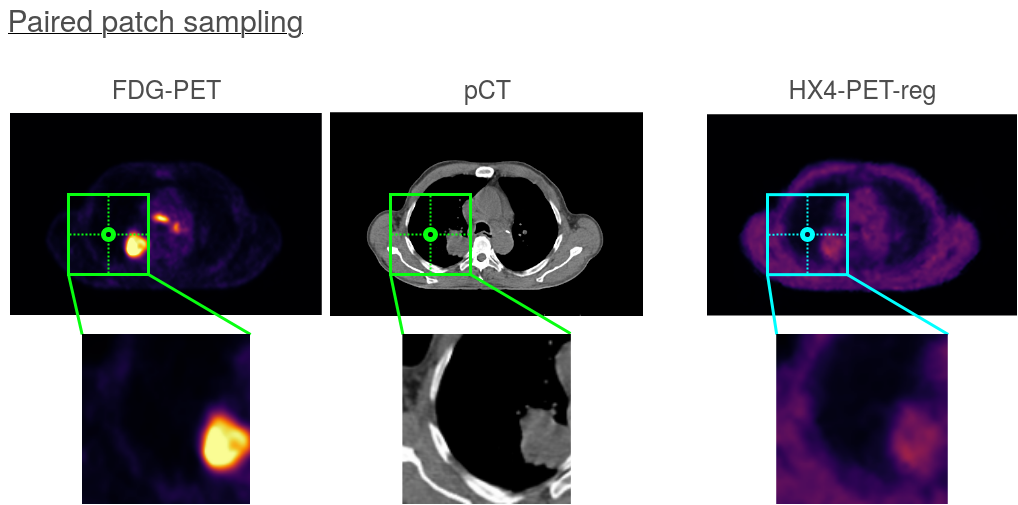
\includegraphics[width=\linewidth]{figures/Data/patch_sampling/paired_patch_sampling.png}
    \caption{Using uniform random sampling in the body region, focal point $f_A$ coordinate (green circles) is first sampled from FDG-PET (and pCT). A corresponding point $f_B$ (cyan circle) is then propagated to HX4-PET-reg such that $f_B = f_A$. Since all three images are spatially aligned, the resulting patches (green and cyan bounding boxes) are aligned as well and cover the same exact anatomical region.}
    \label{fig:paired_patch_sampling}
\end{figure}

In case of unpaired training, a more sensible patch propagation strategy is used instead of sampling patches randomly and independently from the input images and the target domain's unregistered images. The idea is to create a form of ``weak pairing" between the two sets of patches like so -- the anatomical region covered in the input image patches and the HX4-PET-unreg patch should be roughly similar, even though the the input and the target domain images correspond to two different patients. We exploit the fact that all scans have the same patient orientation and a similar FOV. Given the focal point $f_A$ of the patch sampled from the input images, an equivalent focal point $f_B$ is estimated on the HX4-PET-unreg as shown in Equation \ref{eq:unpaired_patch_sampling}.
\begin{equation}
    f_B = \frac{f_A}{size_A} size_B
    \label{eq:unpaired_patch_sampling}
\end{equation}
$f_B$ is calculated such that its relative position with respect to the volume size $size_B$ of the HX4-PET-unreg image is same as the relative position of $f_A$ with respect to the size $size_A$ of the input images. This is then followed by defining a \textit{local sampling region} of size $l_x \times l_y \times l_z$ around $f_B$ and then updating $f_B$ by randomly sampling from this local sampling region. Let this new focal point be denoted as $f_B'$. Again, the condition is applied on $f_B'$ that it must lie within the patient's body region and not in the image background. This additional stochasticity is introduced in the process to account for possible variation in the body position and anatomy across patients. When using ldCT-unreg (i.e. during CycleGAN-balanced training), it shares the same $f_B'$ as HX4-PET-unreg. Figure \ref{fig:unpaired_patch_sampling} shows a visual representation of the unpaired patch sampling process.

\begin{figure}[h!]
    \centering
    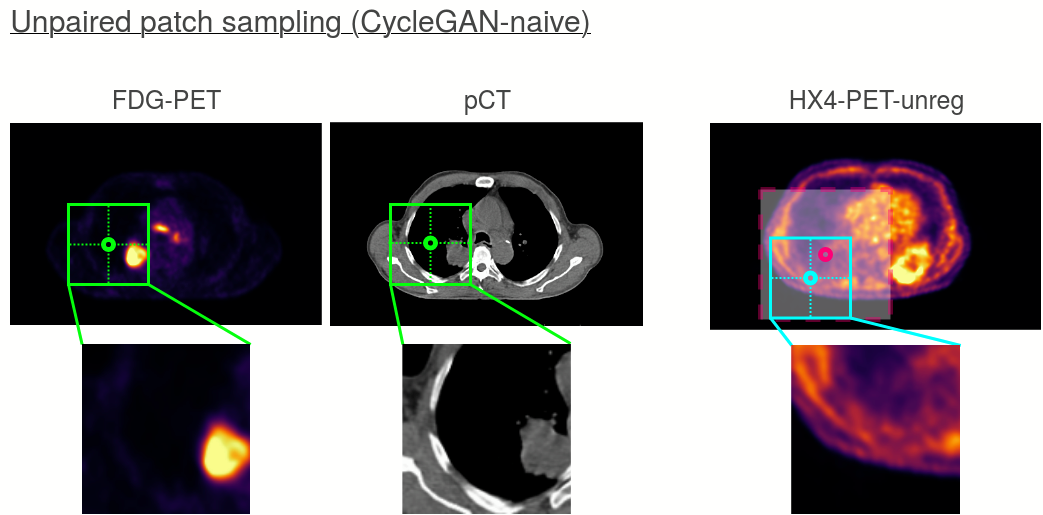
\includegraphics[width=\linewidth]{figures/Data/patch_sampling/unpaired_patch_sampling.png}
    \caption{Given a focal point $f_A$ (green circles) in the input images, a point $f_B$ (pink circle) is propagated to the HX4-PET-unreg image and a local sampling region (pink translucent bounding box) is defined around it. A new point $f_B'$ (cyan circle) is then sampled from this local region and is used to define the HX4-PET-unreg patch (cyan bounding box). Both sets of patches cover similar anatomical regions, despite belonging to images of two different patients.}
    \label{fig:unpaired_patch_sampling}
\end{figure}

The local sampling region is specified as a fraction of the volume size of HX4-PET-unreg image, and in our experiments, we use size 35\% $\times$ 35\% $\times$ 60\%. This relatively large size is set to provide just sufficient freedom for a set of valid patches to be sampled from the full images. A similar, yet much simpler, 2D slice-based unpaired patch sampling was previously suggested by Yang et al. \cite{yang2018unpaired} which produced better results compared to randomly and independently selecting slices for training. We use a fixed patch size of 128$\times$128$\times$32 voxels in both paired and unpaired cases.


\subsubsection{Patch-based validation}
A patch-based inference is used during the model validation phase using a \textit{sliding window} scheme \footnote{Sliding window inferer: \url{https://docs.monai.io/en/latest/inferers.html}}. The same patch size as used in training is used here as well. Given a pair of full-size input images, overlapping patches are sequentially extracted and fed into the GAN model independently. Their corresponding predicted HX4-PET-syn patches are then stitched together into the full-size HX4-PET-syn image. Following this, various image similarity metrics (discussed further in \ref{image_quality_metrics}) are computed between this HX4-PET-syn image and its ground truth HX4-PET-reg. We rescale the predicted and the ground truth images back to their prior intensity scale ($\frac{SUV}{SUV_{aorta-mean}}$ ratio) before computing the metrics. The HX4-PET-syn images are then converted back into SUV intensity representation and saved as NRRD files for later inspection.



%%%%%%%%%%%%%%%%%%%%%%%%%%%%%%%%%%%%%%%%%%%%%%%%%%%%%%%%%%%%%%%%%%%%%%%%%%%%%%%%%%%%%%%%%%%%%%%%%%%%%%%%%%%%%%%%%%%%%%%%%%%%%%%%%%%%%%%%%%%%%%%
\section{Evaluation Methods}
\label{Evaluation_Methods}
The validation set used to track model generalizability is the same data used for final evaluation. We perform an evaluation on the predicted HX4-PET-syn from two different perspectives. In the first, the objective is to evaluate the overall success of the models in learning the input-target mapping, and the evaluation is performed by assessing the fidelity of the full synthetic samples produced by the models with respect to the ground truth. The second perspective regards the clinical value of the synthetic hypoxia maps as the most important factor since the clinical utility of the models is the end goal. In a clinical scenario, the tumor is the sole region-of-interest (ROI) whose hypoxia distribution needs to be measured, and therefore, the evaluation is limited to this locality and consists of relevant application-specific downstream tasks. All metrics are applied on images with intensities expressed in the aorta-normalized SUV ($\frac{SUV}{SUV_{aorta-mean}}$) scale which is clipped to the interval [0, 3]. 


% --------------------------------
\subsection{Image Quality Metrics}
\label{image_quality_metrics}
Isola et al. \cite{isola2017image} note that since Pix2Pix (and this would apply to CycleGAN by extension) learns a structured loss via its discriminator, using simple pixel-wise difference metrics such as mean-squared error is not an effective evaluation strategy, especially for graphics tasks using natural images. Such metrics do not take into account the image statistics and texture the model has learned. However, in the case of quantitative medical images where intensities have some standard scale, element-wise differences can be a meaningful choice and could at least partially be informative about the image quality. We use the following three voxel-wise metrics:

\begin{enumerate}
    \item Mean-Squared Error (MSE): MSE measures the average square of the distances of predicted intensities from the true values. It is more sensitive to large errors. The MSE values are represented in the squared scale of the image intensities and are in the range [0, 9] in our case. Voxel-wise similar images have low MSE.
    \item Mean-Absolute Error (MAE): It measures absolute deviations from the true value and is therefore more robust to outliers as compared to MSE. MAE is reported on the same scale as the image intensities.
    \item Peak Signal-to-Noise Ratio (PSNR): PSNR is a measure related to signal power and is specified in decibels. It is related to MSE in that the ``noise" part in PSNR corresponds to MSE measured with respect to the ``peak signal" which corresponds to the maximum intensity value in the reference image. A higher PSNR value signifies higher quality image in a voxel-wise sense.
\end{enumerate}

We use three additional metrics that measure the statistical properties of a given image in order to complement the ones based on voxel-wise difference. Like the previous three metrics, each of these is a full-reference metric requiring a ground truth reference image. They are given as follows:

\begin{enumerate}
    
    \item Structural Similarity Index Measurement (SSIM): SSIM \cite{wang2004image} is a perceptual metric that focuses on gauging the similarity of perceived local structure between the sample and reference images. It has a fixed scale with a range [-1, 1], -1 being the worst score and 1 being the best which is observed when both images are identical.
    
    \item Normalized Mutual Information (NMI): NMI \cite{studholme1999overlap} is a variant of the mutual information (MI) metric commonly used in multimodal image registration as an image similarity measure. It is an information theoretic quantity which, intuitively, measures the certainty of predicting intensity values in a region of a sample image knowing the intensities of the reference image in the same region. MI indicates the amount of information shared between the two images, and is maximum (1 in case of NMI) when the images are perfectly correlated and is minimum (0 in case of NMI) when they have no correlation. Given a sample synthetic image $\vb{\hat{y}}$ and its corresponding ground truth $\vb{y}$, NMI is calculated as: 
    \begin{equation}
        NMI(\vb{y}, \vb{\hat{y}}) = \frac{H(\vb{y}) + H(\vb{\hat{y}})}{H(\vb{y}, \vb{\hat{y}})}
        \label{eq:metric_nmi}
    \end{equation}
    where $H(\vb{y})$ and $H(\vb{\hat{y}})$ are marginal entropy values for $\vb{y}$  and $\vb{\hat{y}}$, and $H(\vb{y}, \vb{\hat{y}})$ is their joint entropy.
    
    \item Image histogram distance: Histogram distance between two images measures the overlap of their intensity distributions, and has been used as an image similarity measure in applications such as image retrieval. Two identical images would have identical histograms and therefore the distance between the histogram vectors would be 0. However, a drawback of this measure applied on global histograms is that it is unaware of any structures in the images. As an image quality metric, we specifically compute the $\chi^2$ distance between the global histograms of a synthetic image and its ground truth as follows: 
    \begin{equation}
        \chi^2(\vb{h}, \vb{\hat{h}}) = \frac{1}{2} \sum_{b} \frac{[\vb{h}_b - \vb{\hat{h}}_b]^2}{\vb{h}_b + \vb{\hat{h}}_b}
        \label{eq:metric_histogram}
    \end{equation}
    where $\vb{h}$ are $\vb{\hat{h}}$ are histograms of the ground truth and synthetic images, respectively, and $b$ denotes a histogram bin.
    
\end{enumerate}

The idea behind using a set of six metrics for image quality assessment is that each of these metrics has its unique strengths and drawbacks and that we hope of them to complement each other, thereby comprehensively capturing the notion of image quality. The same metrics are used to track model generalizability during training as well. During the evaluation of the final fully-trained models, this set of metrics is used to derive the performance ranking of the models. One could think of the models as candidates in an election and the metrics as the voters, each of which provides a ranking of the models. In this view, the global performance ranking is then derived using the Borda voting scheme.


% ------------------------------------
\subsection{Downstream Image Analysis}
As clinical analysis of the HX4-PET-syn images, we quantify the predicted tumor hypoxia via two downstream tasks -- hypoxic tumor classification and hypoxic region segmentation. The hypoxic tumor classification task involves classifying a tumor as hypoxic or non-hypoxic and thus yields a relatively ``weak" yet robust measure of tumor hypoxia. Knowing the hypoxic status of a tumor during radiotherapy, clinicians can choose to adjust the overall radiation dose to the tumor by increasing the dosage if the tumor is hypoxic. On the other hand, the task of segmenting precisely the exact hypoxic region inside the tumor yields a ``stronger", although less robust, hypoxia measurement. When the exact 3D spatial pattern of the high-hypoxia area is known, the radiation beam can be shaped such that a higher radiation dose is delivered to this area. In addition to the two downstream tasks, the MSE and SSIM metrics are computed locally inside the primary tumor to measure the similarity of the predicted tumor hypoxia distribution with the ground truth. 



%%%%%%%%%%%%%%%%%%%%%%%%%%%%%%%%%%%%%%%%%%%%%%%%%%%%%%%%%%%%%%%%%%%%%%%%%%%%%%%%%%%%%%%%%%%%%%%%%%%%%%%%%%%%%%%%%%%%%%%%%%%%%%%%%%%%%%%%%%%%%%%
\section{A Simulated Problem: Depth Estimation from Multimodal Input}
\label{ClearGrasp_Depth_Estimation}

Pix2Pix and CycleGAN are general frameworks capable of being applied to a large space of image translation problems without much modification. On the other hand, the altered design of the CycleGAN-balanced system is meant to be problem-specific and optimized for our use case. Either way, testing the different GAN approaches on medical imaging data is difficult for several reasons -- (1) training GANs on 3D images is time-consuming, (2) special visualization software is required to inspect the predicted 3D images, and (3) certain failure modes and artifacts in the medical images can be hard to detect for an untrained observer. Therefore, it is extremely difficult to identify any existing methodological flaws or implementation bugs that may propagate into the results, thereby leading to misinterpretation. To rapidly and effectively prototype, debug and test the GANs, we construct a simple 2D image-to-image translation task inspired by computer vision literature that is also representative of the challenges of our medical image translation task. This simulated computer vision task involves estimation of depth from a multimodal input comprised of color photographs and surface normals, and the dataset we use is the ClearGrasp dataset of transparent objects \cite{sajjan2020clear}.

ClearGrasp is a publicly available dataset \footnote{ClearGrasp website: \url{https://sites.google.com/view/cleargrasp/synthetic-dataset}} for benchmarking deep-learning-based monocular depth estimation (and depth completion) methods in challenging environments where transparent objects are the objects of interest. It contains 50,000 training samples and 532 validation samples representing five different transparent objects. Each sample is a set of synthetic 2D images consisting of different spatially aligned renderings, including a color photograph, a depthmap, a surface normal map, segmentation masks, and object outlines. Of main interest to us are the first three since they essentially correspond to different modalities that contain complementary information. Figure \ref{fig:cleargrasp_sample} visualizes a sample set of these images. 

\begin{figure}[h!]
    \centering
    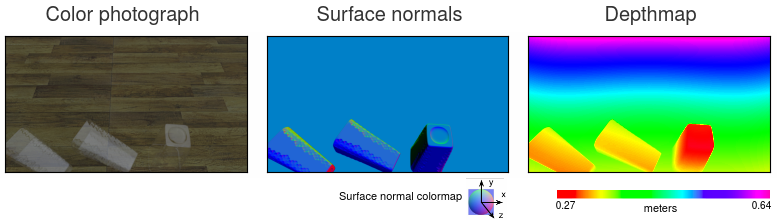
\includegraphics[width=\linewidth]{figures/Cleargrasp_data/cleargrasp_sample.png}
    \caption{Transparent objects are difficult to delineate in the color photograph since their surfaces are not distinctly visible. Furthermore, estimating depth precisely from merely one monocular color photo is a challenging problem by itself. However, given explicitly the information on the surfaces in the scene, estimation of depth of transparent objects becomes much more approachable.}
    \label{fig:cleargrasp_sample}
\end{figure}{}

We argue that this depth estimation task can simulate up to a certain extent the challenges of the HX4-PET prediction task. Following is an analysis of the involved modalities and the analogy between the two translation tasks:
 
\begin{enumerate}
    
    \item Color photograph: This modality captures the optical properties of a scene including the shades of colors on various objects and the shadows and reflections cast by the objects. Using these features, one can differentiate one object from the other and can perceive their 3D structure. However, transparent objects are difficult to delineate when relying solely on optical information due to the refractive property of their surfaces. The role of a photograph in this depth estimation task can be viewed as being analogous to the role of pCT in hypoxia map prediction problem, since both the modalities supply rich structural information regarding the overall scene but fail to be informative about one specific region -- transparent objects' structure in case of photograph image and tumor biology in case of pCT.
    
    \item Surface normals: Surface normal images encode information about 3D surface angles into a 2D image via a colormap. In the ClearGrasp dataset, surface normal renderings explicitly supply precise surface data, even for transparent objects. Therefore, this modality provides an additional layer of information that complements photographic images. Surface normals, however, fail to differentiate between parallel surfaces even when the surfaces are at different depths from the observer. In contrast, a photograph can be useful in such a situation depending on the lighting conditions. Both modalities are, therefore, mutually complementary. Surface normal image is then analogous to FDG-PET in the sense that both are informative about certain regions in the scene which their respective structural image modalities (color photograph and pCT) fail to capture, although each of them on their own is not sufficient for their respective task. 
    
    \item Depthmap: Depthmaps are single-channel 2D images whose pixel intensities represent the distance of the scene elements from the camera and are the target image modality in the simulated problem task. It has a mathematical relationship with surface normals since both are ``quantitative" images whose intensities represent some physical property. In fact, the latter can be computed from the former directly using gradients of the depth values \footnote{Algorithm for computing surface normals from depthmap: \url{https://bit.ly/3mQS588.}}. For our purpose, the depthmap serves an analogous role to HX4-PET in that tumor hypoxia is closely related to metabolism, a relationship that is physiological in nature.
    
\end{enumerate}

Using the equivalent 2D architecture of their 3D generator and discriminator networks, we apply the same three GAN systems -- Pix2Pix, CycleGAN-naive, and CycleGAN-balanced -- on this simulated problem task to obtain a prior estimation of their relative performance. In CycleGAN-balanced training, to serve a role that is analogous to ldCT-unreg in the HX4-PET synthesis task, photographic images corrupted with added Gaussian noise are used as the structural context images for their corresponding depthmaps.

A small-scale dataset for this simulated task is curated as a subset of the larger ClearGrasp set. Out of the five types of transparent objects whose images the original dataset contains, we limit our data to one object type which has a relatively simple structure -- the ``square plastic bottle". From the dataset, we select 25,000 training samples and 100 validation samples corresponding to this object to compose the subset. Each sample consists of a color photograph, a surface normal image, and a depthmap.